\documentclass[eng,printmode, openany]{mgr}
\usepackage{listings}
\usepackage[english, polish]{babel}
\usepackage{graphicx}
\usepackage{hyperref}
\usepackage{tabularx,colortbl} 
\usepackage{rotating}
\usepackage{polski}
\usepackage[utf8]{inputenc} 
\setlength\parindent{24pt}
\usepackage[parfill]{parskip}
\usepackage{listings}
\usepackage[table,kernelfbox,hyperref]{xcolor}
\usepackage[xindy]{glossaries}
\usepackage{fancyhdr}
\usepackage{amsmath}
\usepackage{subfig}

%\usepackage[colorinlistoftodos]{todonotes}

\hypersetup{colorlinks=true}
\hypersetup{xurlbordercolor=red!70!black}
\hypersetup{xlinkbordercolor=blue!70!black}
\hypersetup{linkcolor=blue!60!black}
\hypersetup{urlcolor=red!50!black}
\hypersetup{citecolor=green!30!black}
\makeglossaries
\rfoot{Page \thepage}
\renewcommand\lstlistlistingname{List of Listings}
\newcommand{\linia}{\rule{\linewidth}{0.4mm}}

\definecolor{listlightgray}{gray}{0.93}

\newcommand{\lstsetmylst} {
	\lstset{frame = tb,
		breaklines=true,
		framerule = 0.25pt,
		float,
		fontadjust,
		backgroundcolor={\color{listlightgray}},
		basicstyle = {\ttfamily\footnotesize},
		identifierstyle = {\ttfamily},
		stringstyle = {\ttfamily},
		showstringspaces = false,
		showtabs = false,
		numbers = left,
		numbersep = 6pt,
		tabsize = 4,
		language=C,
		floatplacement=!h
	}
}

\newcommand{\lstsetatc} {
	\lstset{frame = tb,
		breaklines=true,
		framerule = 0.25pt,
		float,
		fontadjust,
		backgroundcolor={\color{listlightgray}},
		basicstyle = {\ttfamily\footnotesize},
		keywordstyle = {\ttfamily\color{listkeyword}\textbf},
		identifierstyle = {\ttfamily},
		commentstyle = {\ttfamily\color{listcomment}\textit},
		stringstyle = {\ttfamily},
		showstringspaces = false,
		showtabs = false,
		numbers = left,
		numbersep = 6pt,
		numberstyle={\ttfamily\color{listnumbers}},
		tabsize = 4,
		language=C,
		floatplacement=!h
	}
}

\newcommand{\lstsetatbashnum} {
	\lstset{frame = tb,
		breaklines=true,
		framerule = 0.25pt,
		aboveskip=2ex,
		float,
		fontadjust,
		backgroundcolor={\color{listlightgray}},
		basicstyle = {\ttfamily\footnotesize},
		keywordstyle = {\ttfamily\color{listkeyword}\textbf},
		identifierstyle = {\ttfamily},
		commentstyle = {\ttfamily\color{listcomment}\textit},
		stringstyle = {\ttfamily},
		showstringspaces = false,
		showtabs = false,
		numbers = left,
		numbersep = 6pt,
		numberstyle={\ttfamily\color{listnumbers}},
		tabsize = 4,
		language=bash,
		floatplacement=!h
	}
}
\author{Adam Superczyński,\\Jarosław M. Szumega}
\title{Data conversion path from RS--232 to FSK transmitter. }
\engtitle{}
\supervisor{Grzegorz Budzyń Ph.D., (W4/K-4)}
\field{Electronics Engineering}
\specialisation{Advanced Applied Electronics}
\date{2018}
\begin{document}
	\selectlanguage{english}
	\maketitle
	\tableofcontents
\chapter{Project description}
The goal of the following project is to design and prepare the hardware realization of the circuit able to convert RS--232 data to FSK (FM modulation).\\
\\
To achieve this result, the following assumptions were made:
\begin{itemize}
	\item data to be transmitted will be send from PC to RS--232 interface,
	\item the data preparation will be achieved utilizing ARM microcontroller (RS--232 receiving, generating carrier wave, modulating the signal),
	\item additional analogue circuit will be designed and assembled to perform all necessary signal post--processing (e.g. amplification).
\end{itemize}
\chapter{Design and simulation}

The digital part (microcontroller) is responsible for receiving the RS--232 data and performing carrier generation and signal modulation.

%Pan Adam
It was done by [...]

%Pan Adam
On the other hand, the analogue circuit deals with [...]

The complete design was prepared in LTSpice, that also allowed to perform a simulations of the circuit.
\begin{figure}[h]
	\centering
	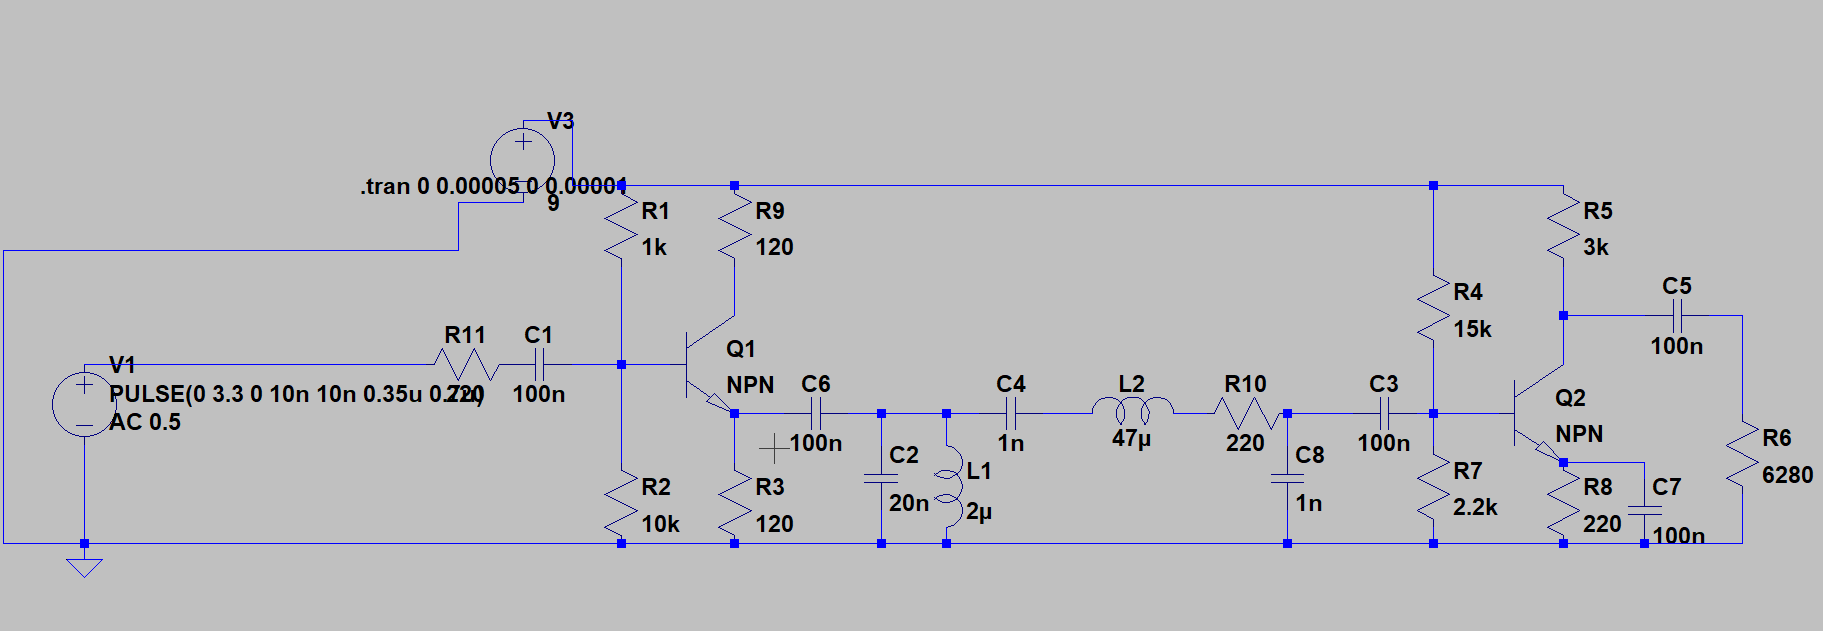
\includegraphics[width=0.9\linewidth]{design}
	\caption{LTSpice desing of analogue part.}
	\label{fig:design}
\end{figure}
\begin{figure}[h]
	\centering
	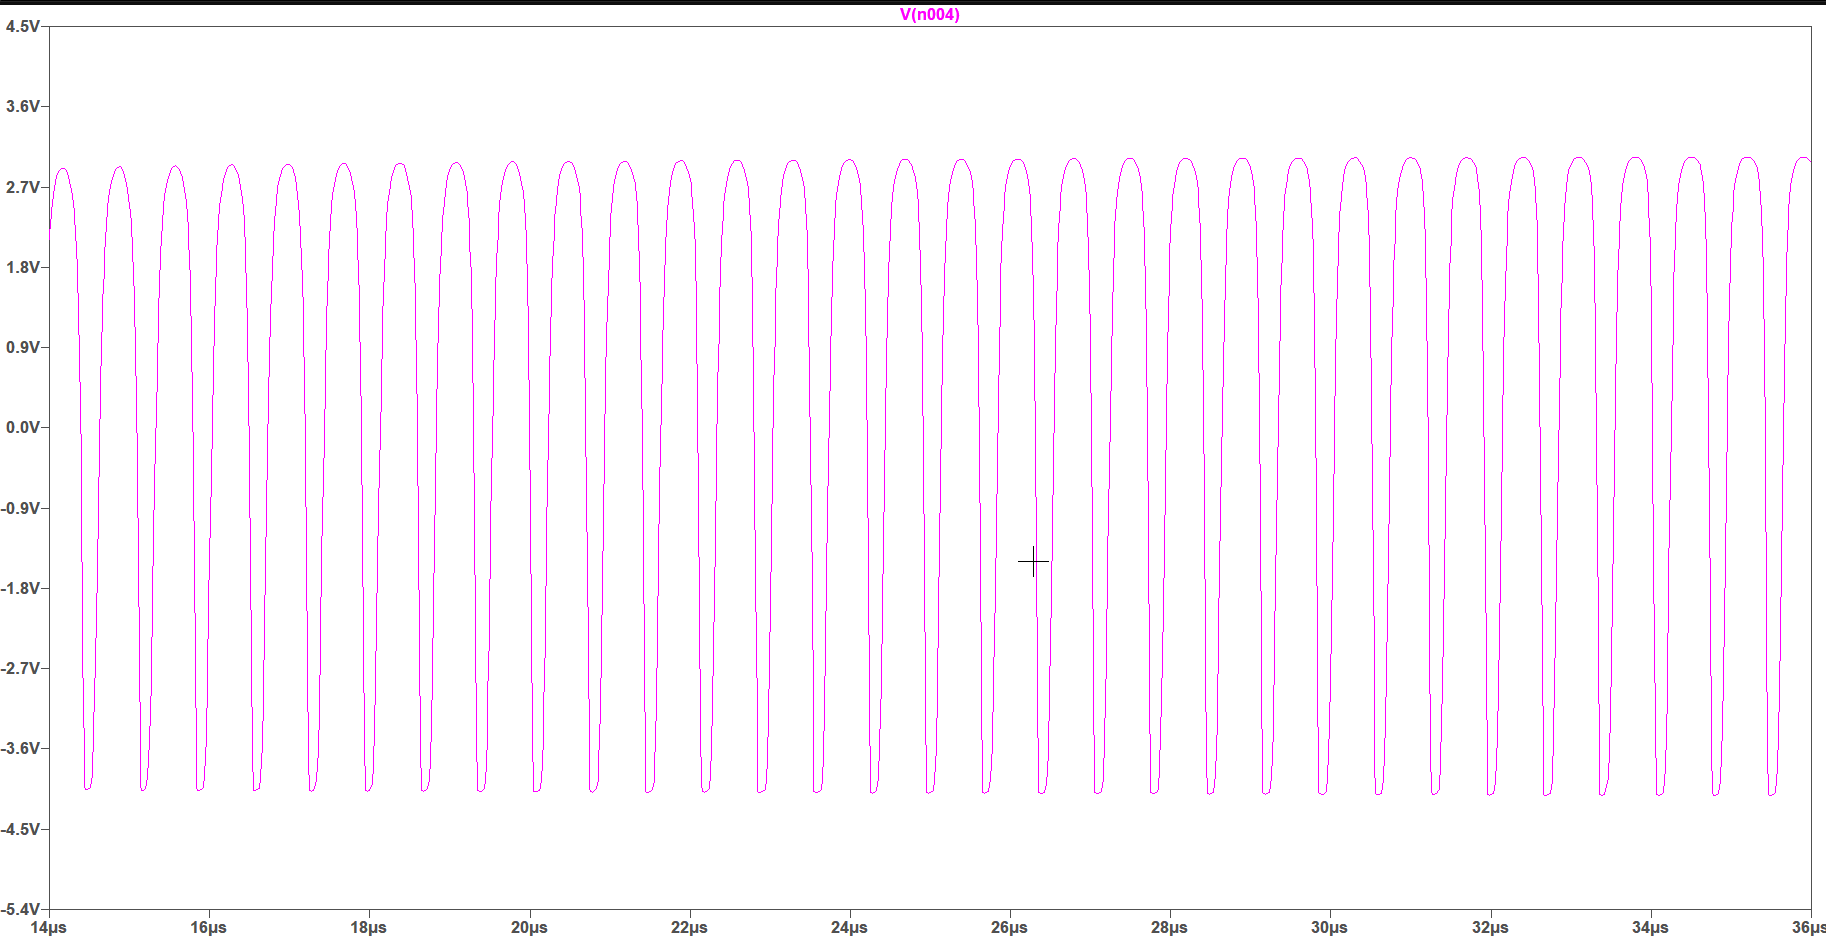
\includegraphics[width=0.7\linewidth]{output}
	\caption{Simulated output of the final stage of amplification.}
	\label{fig:output}
\end{figure}

\chapter{Physical realization}

%Pan Adam fotki i spis elementów

\begin{figure}
	\centering
	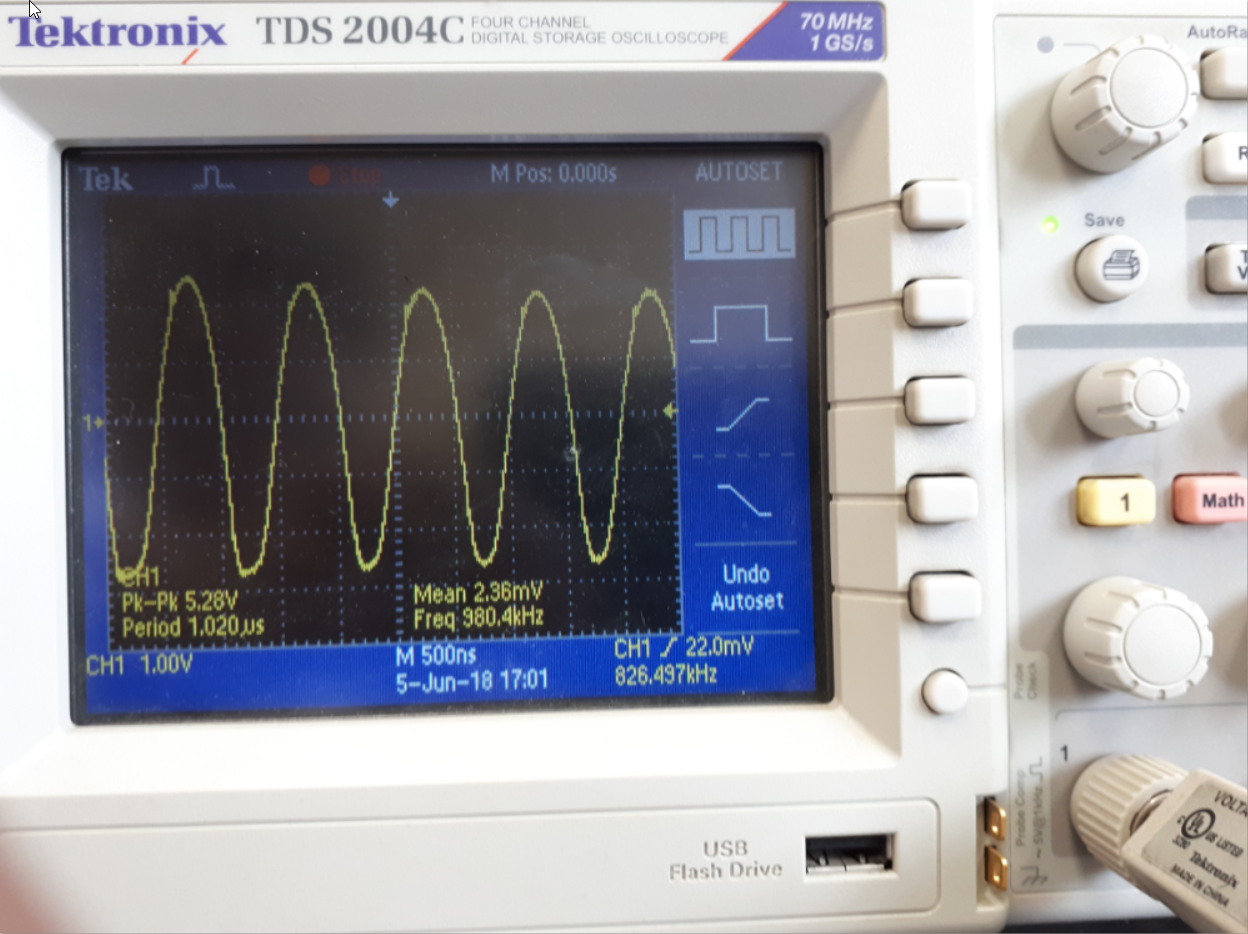
\includegraphics[width=0.7\linewidth]{output1}
	\vspace{20pt}
	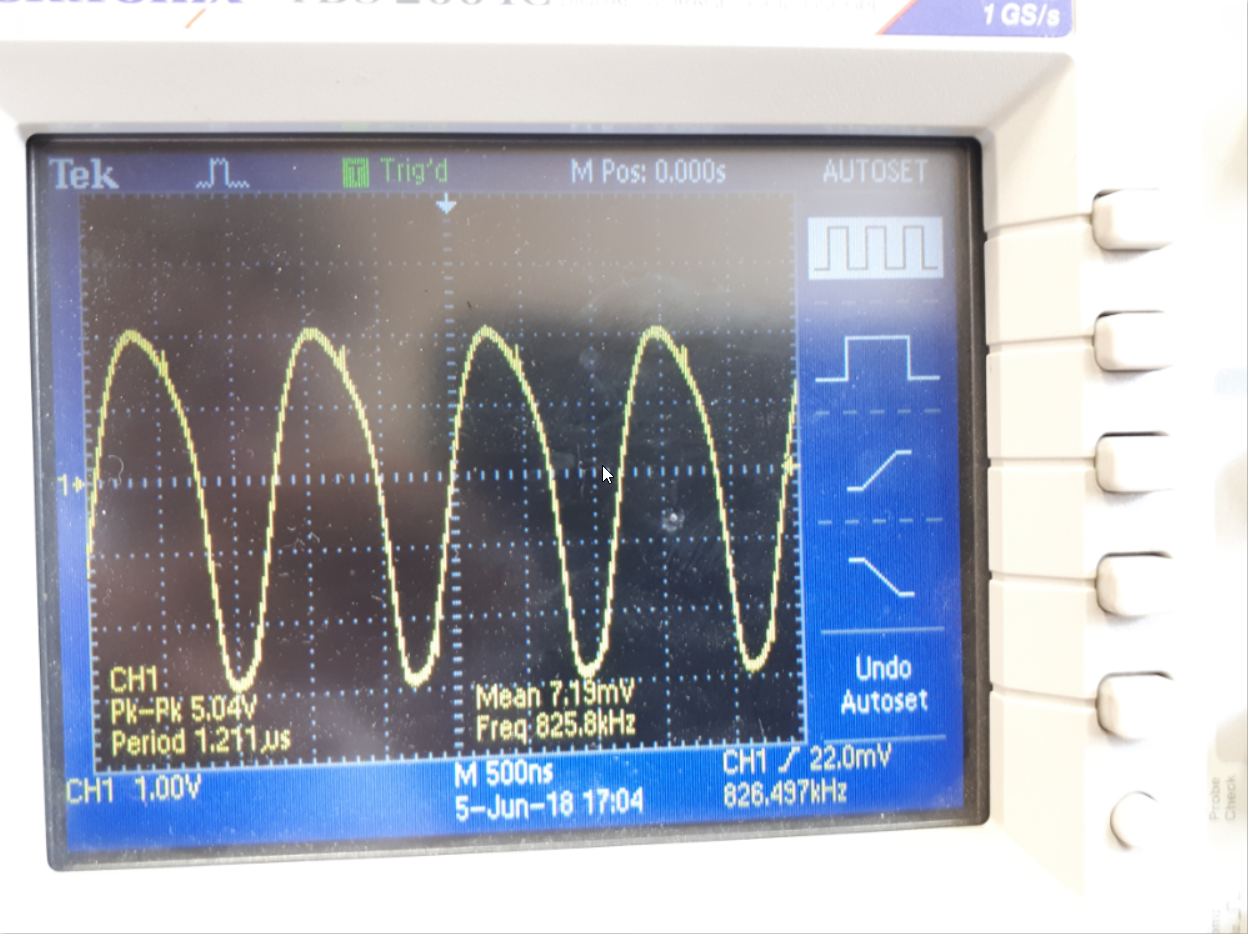
\includegraphics[width=0.7\linewidth]{output2}
	\caption{Frequency modulation presented at analog circuit output (825 and 980 kHz)}
	\label{fig:output1}
	
\end{figure}

\chapter{Conclusions}

%a to w ogóle potrzebne?
\begin{thebibliography}{9}

\end{thebibliography}
	
\end{document}